\documentclass[xcolor=dvipsnames]{beamer}

% Ausgelagerte Praeambel
\mode<presentation> {
   \usetheme{Copenhagen}
   \usecolortheme[named=PineGreen]{structure}
   \setbeamercovered{dynamic}
}

% Sprache und Zeichnsatz
\usepackage[ngerman]{babel} 
\usepackage[latin1]{inputenc}

% font definitions, try \usepackage{ae} instead of the following
% three lines if you don't like this look
\usepackage{mathptmx}
\usepackage[scaled=.90]{helvet}
\usepackage{courier}

% Um Bilder einzufuegen
\usepackage{graphicx} 

\usepackage[T1]{fontenc}

% Titelseiteninformationen
\author[Lukas Ehnle, Jo Klawitter, 
Nikos Moraitakis, Alex Noe, Anas Saber]{Lukas Ehnle, 
Jo Klawitter, Nikos Moraitakis, Alex Noe, Anas Saber}
\institute{KIT, Fakult�t f�r Informatik}
\date{\today} 

 
% This is only inserted into the PDF information catalog. 
\subject{Tutoriumsfolien}
\keywords{PSE10, Research Phase}


% Logo rechts unten einbinden
\pgfdeclareimage[height=0.8cm]{university-logo}{Pictures/KIT-Logo.png}
\logo{\pgfuseimage{university-logo}}


  
% Abschalten der unteren Symbolleiste:
\beamertemplatenavigationsymbolsempty

% If you wish to uncover everything in a step-wise fashion, uncomment
% the following command:
%\beamerdefaultoverlayspecification{<+->}
 


%<[BEGIN]><[BEGIN]><[BEGIN]><[BEGIN]><[BEGIN]><[BEGIN]><[BEGIN]><[BEGIN]>
\begin{document}  %<[BEGIN]><[BEGIN]><[BEGIN]><[BEGIN]><[BEGIN]><[BEGIN]>
%<[BEGIN]><[BEGIN]><[BEGIN]><[BEGIN]><[BEGIN]><[BEGIN]><[BEGIN]><[BEGIN]>

% :-:-:-[ Starteite ]-:-:-:-:-:-:-:-:-:-:-:-:-:-:-:-:-:-:-:-:-:-:-:
\begin{frame}
\begin{center}
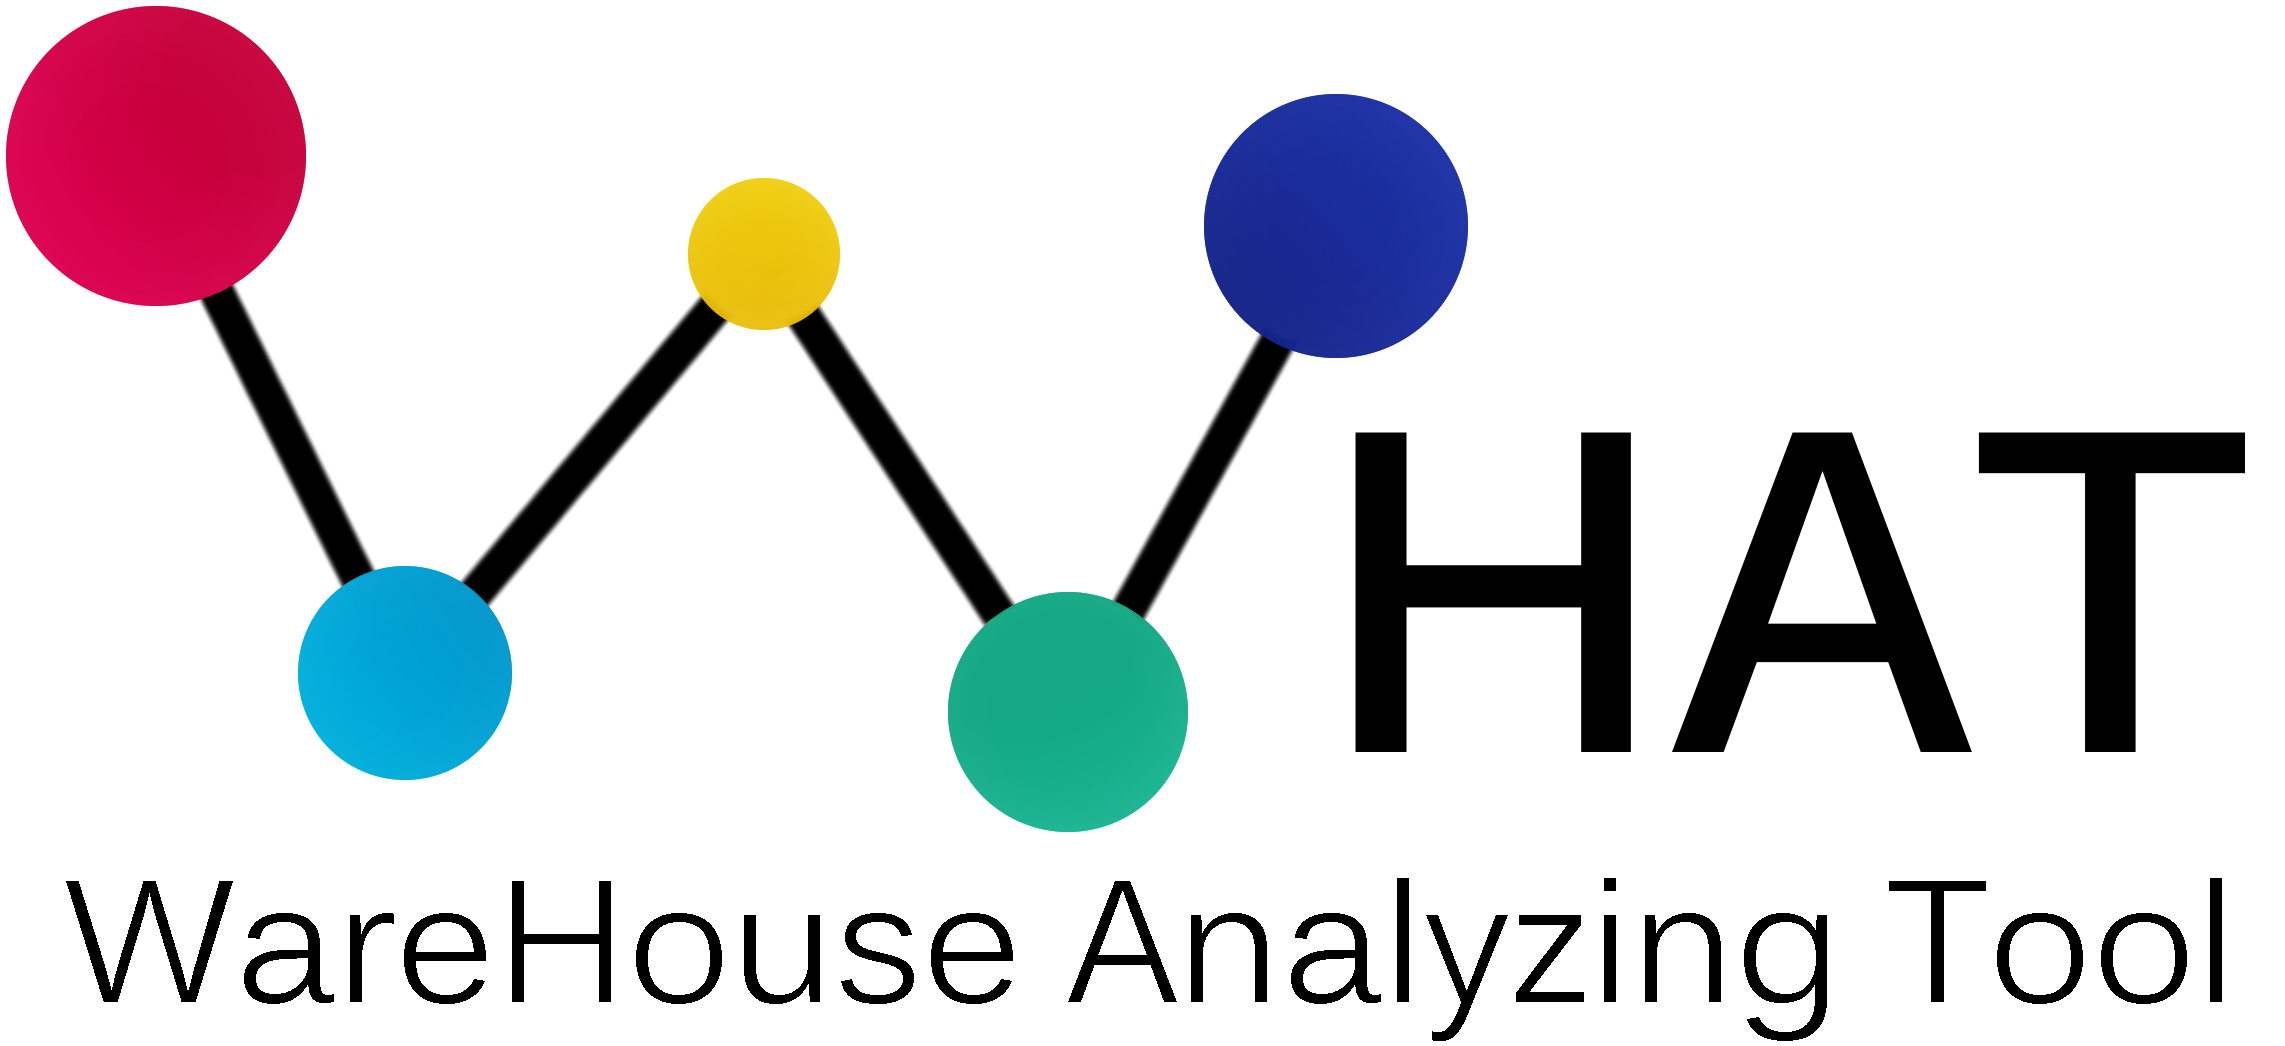
\includegraphics[width =0.7\linewidth]{Pictures/WHAT-Logo2.png}
\end{center}

\end{frame}
% 
% % :-:-:-[ Titelseite ]-:-:-:-:-:-:-:-:-:-:-:-:-:-:-:-:-:-:-:-:-:-:-:
% \begin{frame}
% \titlepage
% \end{frame} 

% % :-:-:-[ Inhaltsverzeichnis ]-:-:-:-:-:-:-:-:-:-:-:-:-:-:-:-:-:-:-:
% \begin{frame}{Content} 
% \tableofcontents%[hideallsubsections]
% \end{frame}


%  - - -[ Folie ]- - - - - - - - - - - - - - - - - - - - - - - - - -
\begin{frame}{Title here}

%\includegraphics[width=1\linewidth]{PicturenameHere.png}

\end{frame}




%  - - -[ Folie ]- - - - - - - - - - - - - - - - - - - - - - - - - -
\begin{frame}{End}

\begin{center}
\huge{Thanks for listening!}
\end{center}


\end{frame}  


%<[END]><[END]><[END]><[END]><[END]><[END]><[END]><[END]><[END]><[END]>
\end{document}       %<[END]><[END]><[END]><[END]><[END]><[END]><[END]>
%<[END]><[END]><[END]><[END]><[END]><[END]><[END]><[END]><[END]><[END]>